%Präambel
\documentclass[paper=a4,fontsize=11pt,headsepline,footsepline,parskip=half]{scrartcl}
\usepackage[utf8]{inputenc}
\usepackage[T1]{fontenc}
\usepackage{amsmath,amsfonts,amssymb}
\usepackage{ngerman,graphicx,textcomp,mathpazo,booktabs}
\usepackage[decimalsymbol=comma,per=frac]{siunitx}
\usepackage[textfont=sl,labelfont=bf]{caption}

%Seite einrichten
\areaset[2cm]		% Zusätzlicher Rand für die Bindung
        {17cm}{24cm}	% Textbreite und -Höhe

%Zeilenabstand
\linespread{1.2} %Standardwert

%Kopf- und Fußzeile
\usepackage{scrlayer-scrpage}
\setlength{\headheight}{23pt}
\lohead{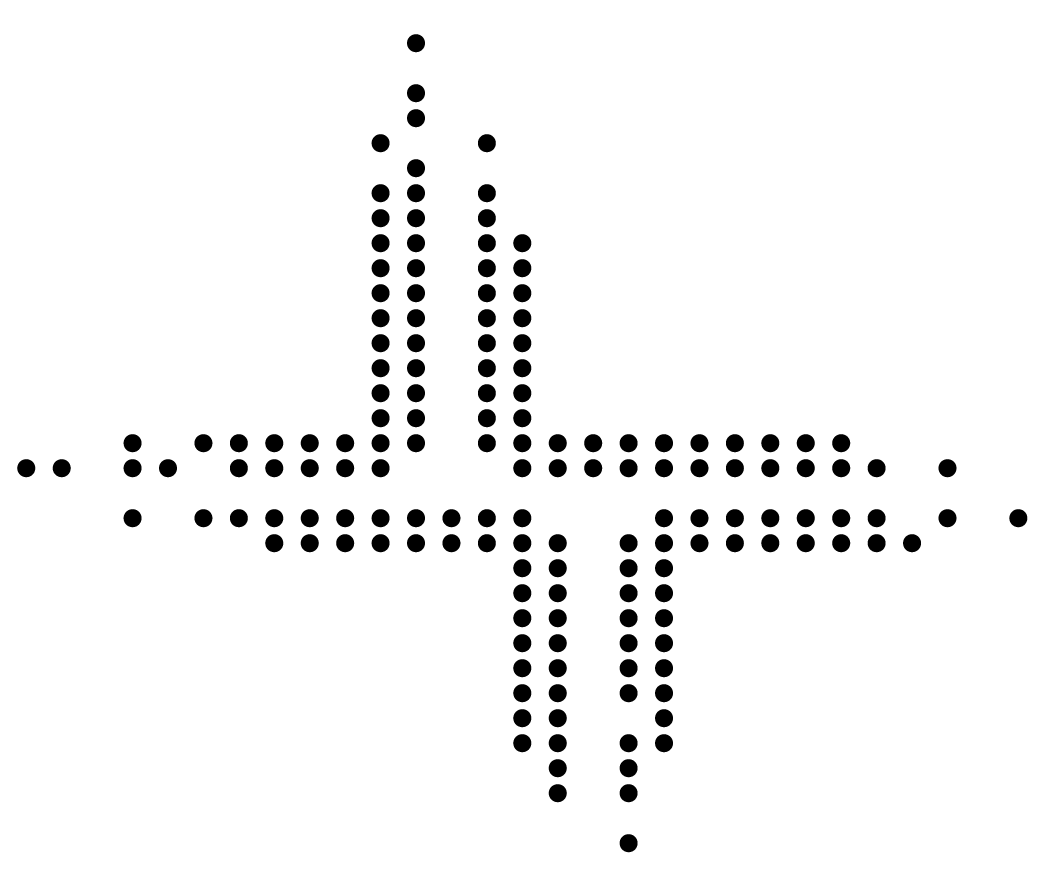
\includegraphics[width=0.7cm]{../logofbi} Hochschule Darmstadt}
\rohead{David Falk, Christian Lichtsinn}
\pagestyle{scrheadings}

%Programmierzeilen
\usepackage{listings}
%Optionen für listings
\lstset{
frame=single, %Rahmen
numbers=left %Zeilennummer
}

%sollte als letztes Paket geladen werden
\usepackage{hyperref}

\begin{document}

%Titelblatt
\begin{titlepage}

\begin{minipage}[c]{5cm}
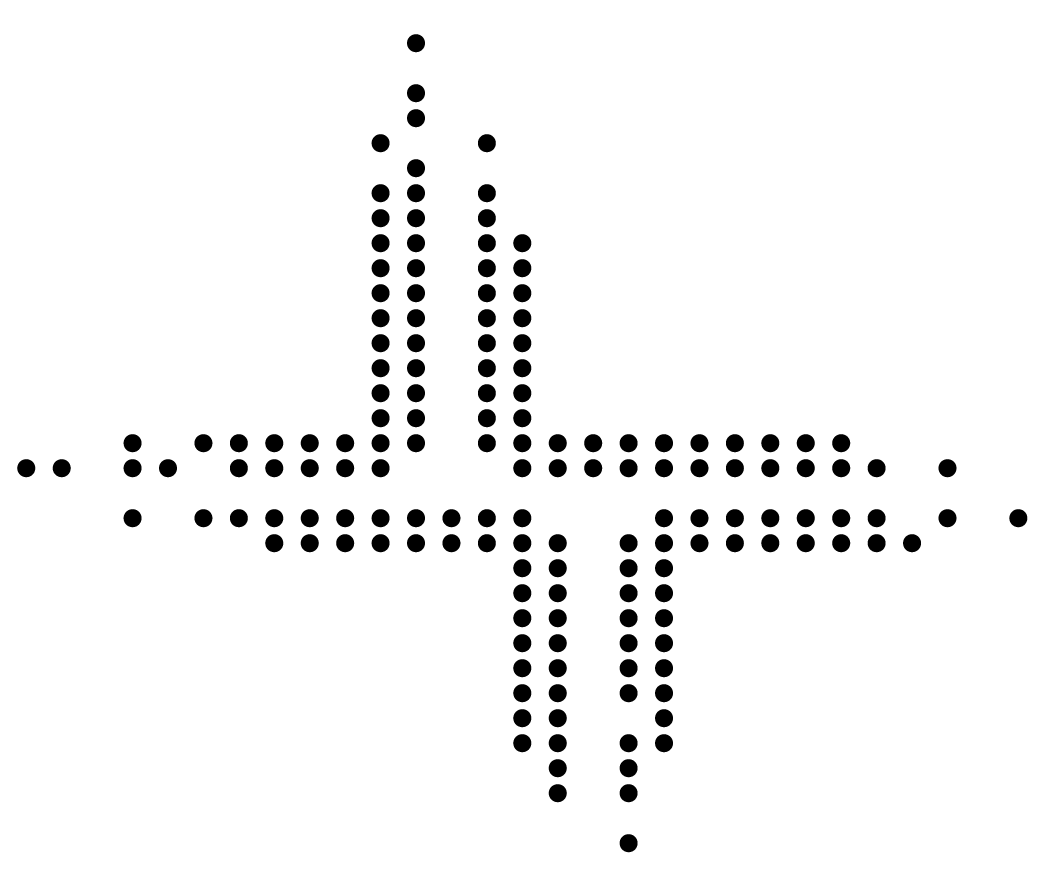
\includegraphics[width=5cm]{../logofbi}
\end{minipage}
\hfill
\begin{minipage}[c]{10cm}
\begin{flushright}
\Large Einführung in die Technik\\und Anwendung von\\
\LARGE \textbf{RFID}
\end{flushright}
\end{minipage}

\vspace*{1cm}

\begin{minipage}[c]{9cm}
\begin{flushleft}
\large David Falk (736532)\\Christian Lichtsinn (736787)\\Praktikum 4: 30.11.15: \textbf{Mo-56x}
\end{flushleft}
\end{minipage}
\hfill
\begin{minipage}[c]{7cm}
\begin{flushright}
\large Betreuer:\\Prof. Ralf S. Mayer\\F. Dotzauer
\end{flushright}
\end{minipage}

\vspace*{1cm}

%Workaround nötig wegen parskip Option.
\begingroup
  \setlength{\parskip}{0pt}% keinen Absatzabstand einfügen
  \setlength{\parindent}{0pt}% nicht einziehen
  \setlength{\parfillskip}{0pt plus 1fil}% Absatz darf komplett gefüllt sein
  \par\rule{\linewidth}{1.5pt}\par
\endgroup

\vspace*{\stretch{1}} %stretch zählt all stretch zusammen (hier 1+2=3) und verteilt den vspace entsprechend, hier 1/3

\centering
\Huge{\textbf{\textsl{HF- und UHF-Leser\\Setup \& Tests}}}

\vspace*{\stretch{2}} %und hier 2/3 vspace vom Rest der Seite.

\end{titlepage}

%KAPITEL 1
\section{Fragen zu HF scemtec}

\subsection{In welchem Frequenzband arbeitet ISO 15693?}

Bei $13,56 MHz$, HF (high frequency).

\subsection{Was versteht man unter STX und ETX bei der seriellen Übertragung zum Gerät?}

STX und ETX sind so etwas wie Funktionsklammern. Sie stehen für \textbf{Start of Transmission} (STX) und \textbf{End of Transmission} und
umschließen einen Funktionsaufruf. Beispiel:

\begin{lstlisting}
 STX "F000" <vv> ETX {c}
\end{lstlisting}

\subsection{Was muss man bei der Zusammensetzung eines Kommandos über serielle Schnittstelle an den scemtec-Reader beachten?}

TODO (Wie das Kommando aufgebaut ist?)

%KAPITEL 2
\section{Fragen zu SamSys-UHF-Reader}

\subsection{Wie ist das Lesegerät MP9320 in Betrieb zu nehmen, was ist zu beachten, wie wird die Antenne angeschlossen?}

Das Lesegerät verbindet man mit einem seriellem Kabel mit einem PC, damit man via einer Software mit dem Lesegerät kommunizieren kann. Das MP9320
darf dabei aber erst in Betrieb genommen werden, wenn entweder an den Antennenanschlüssen entsprechende UHF-RFID-Antennen angeschlossen sind oder
sich ein $50\ohm$-Abschlusswiderstand anstatt der Antenne befindet.

\subsection{Könnten mehrere UHF-Lesegeräte sich gegenseitig beeinflussen?}

Ja, es wird aber versucht dies durch Anti-Kollisionsverfahren zu vermeiden.

\subsection{Was bedeutet ISO 18000-6?}

ISO 18000-6 ist eine Norm für die Spezifikation der Luftschnittstelle im UHF-Bereich (Ultra High Frequency) von $860 MHz$ bis $960 MHz$.

\subsection{Wie können Tags mit der RF Command Suite und der RS232-Schnittstelle gelesen werden?}

TODO

%KAPITEL 3
\section{scemtec}

\section{SamSys}

\end{document}
